%%%
%
% $Autor: Wings $
% $Datum: 2021-05-14 $
% $Pfad: GitLab/MLEdgeComputer $
% $Dateiname: TinyMLExamples 
% $Version: 4620 $
%
% !TeX spellcheck = de_GB
%
%%%

\chapter{Tiny-ML on Arduino Nano 33 BLE Sense}

Machine learning (ML) and Artificial intelligence (AI) are everywhere, its application, use cases and importance make it very usefull for every process. In the same sense, the tiny Arduino nano 33 BLE Sense board give us a way to make Tiny-ML application, where the model are not as big as previuosly made for high and big processing computer. By having a tiny machine learning model we can deploy it on low power devices, one of these is Arduino nano 33 BLE Sense. Due to its small size, the available set of sensors and low power consumption, it is easy to use anywhere by deploying the Machine leaarning algorithm and run the Internet of things (IOT) and Articial intelligence (AI) application for any process.\cite{Dokic:2020}

\section{Usefull Tiny-ML Model for Arduino Nano 33 BLE Sense}

\subsection{Voice Recognition}

Although, being a low power processing device it is not supported the big model and very big data. One of the usefull Tiny-ML model we can make on Arduino Nano 33 BLE Sense is to detect the different voices from the sorrounding. There is a on-board embed sensor on arduino for detecting voices is MP34DT05 the digital microphone. By using the MP34DT05, we can make a data set for keyword voice recognition model. Initially we train a model on Google colab and then convert it into TensorFlow lite for low power devices.\cite{Waqar:2021} For using the Voice recognition functionality of arduino nano 33 ble board, we need the on-board sensor MP34DT05 (Microphone), which is use for capturing, recognizing and detecting the voice. The supporting library for activating this sensor is PDM which will be discussed in the later chapter.

\subsection{Custom Gesture Recognition}

For capturing the gesture data using the on-board 9-axis Inertial measurement unit (IMU), we can make different types of gestures by rotating and changing the position by holding the arduino board in our hand . By doing this, the 9-axis IMU changes the accelerometre, and gyroscope value of the sensor. The limitation for training this model is to hold the board in our hand all the time. But, for the testing purpose it changes the valuse as per the gesture as shown in the figure below \ref{IMU Sensor Capture Data} for training the Tiny-Ml model.\cite{Arduino:2021}

\begin{figure}[ht]
    \centering
    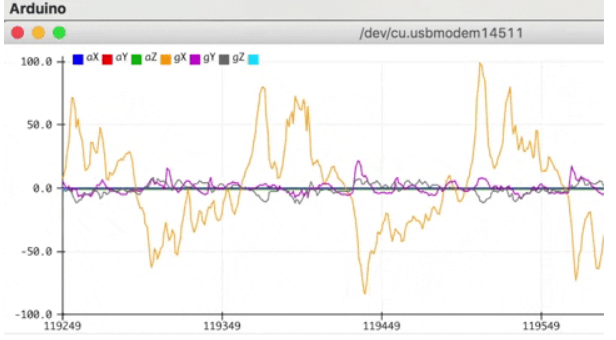
\includegraphics[width=0.5\linewidth]{Nano33BLESense/IMUData}
    \caption{IMU (Inertial Measurement Unit) Gesture Data} 
    \label{IMU Sensor Capture Data}
\end{figure}

The another possibility for detecting gesture is to use the APDS9960 sensor, it can also detect the gesture by moving the hand in front of it. It has also some limitation, it will not detect any gesture above 15 mm distance from the sensor.

\subsection{Color Detection}

The same above mentioned sensor APDS9960 is use for (Red, Green, Blue) RGB color detection too. We can also use the RGB functionality of this sensor and train the Tiny-ML model for detecting the different color product, which make the differentiation among the product on the basis of RGB color.

\subsection{Person Detection} 

One of the advantages of using a small devices such as the Arduino Nano 33 BLE Sense with TinyML is that it could be used as a remote low powered sensor to detect movement or even if there is a person in the area or not. APDS9960 sensor working as a proximity sensor, it can start to detect person at the certain distance. For doing this, we need external camera which can detect the moving person in the sorrounding or not. The supporting camera can be a Arducam Mini 2MP, which will be discuused in the hardware setup chapter later. Some usefull libraries e.g; JPEGDecoder library to decode JPEG-encoded images, the Arducam Library  need to be installed to make the compatibility between Arducam and edge computer (Arduino Nano 33 BLE Sense) by setting the hardware parametre in the library folder. The most necassary setting will be discussed in the later chapters too. \href{https://www.element14.com/community/community/project14/nano-rama/blog/2020/04/29/tinyml-on-arduino-nano-33-ble-sense-person-detection-with-ble}{Person Detection}

